\documentclass{beamer}
\usetheme{Madrid}
\usepackage[utf8]{inputenc}
\usepackage[spanish]{babel}
\usepackage{xspace}
\usepackage{amsmath}
\usepackage{tikz}
\usetikzlibrary{arrows,positioning,shapes,shadows,fit}
\usepackage{graphics}
\usepackage{xcolor}
\usepackage[beamer]{hf-tikz}
\usepackage{bussproofs}

\usefonttheme{serif}

%\usepackage{soul}
%\makeatletter
%\let\HL\hl
%\renewcommand\hl{
    %\let\set@color\beamerorig@set@color
    %\let\reset@color\beamerorig@reset@color
    %\HL}
%\makeatother
%\newcommand{\mathcolorbox}[2]{\colorbox{#1}{$\displaystyle #2}}

\usepackage{xcolor}
\definecolor{gray97}{gray}{.97}
\definecolor{gray75}{gray}{.75}
\definecolor{gray45}{gray}{.45}
\definecolor{gray90}{gray}{.92}

\usepackage{listings}
\lstdefinestyle{CodigoC}
{basicstyle=\tiny\ttfamily,
	frame=single,
	language=C,
	numbers=left,
	numbersep=6pt,
	numberstyle=\tiny,
	framexleftmargin=0.4cm,
	backgroundcolor=\color{gray90},
	keywordstyle=\bfseries
}

\usepackage{pgfplots}
\pgfplotsset{compat=1.16}

\lstdefinestyle{plain-text}
{
	backgroundcolor=\color{white},
	%basicstyle=\ttfamily\small,
	basicstyle=\tiny\ttfamily,
	numbers=none,
	frame=single
}
\newcommand{\chcir}{CHC-IR }
\newcommand{\bubble}{\texttt{bubble\_sort}\xspace}
\usepackage{caption}
\usepackage{subcaption}
\AtBeginSection[]

\newcommand\Idris{\textsc{Idris}}
\newcommand{\dsltitle}{Example - Modelling an ATM DSL in Idris}
\newcommand{\othertitle}{Example - Other}

\title{\Idris, a general-purpose dependently typed programming language: Design and implementation -- Edwin Brady}
\author{Daniela Ferreiro, Jorge Blázquez, Daniel Trujillo, Rafael Fernández}
\date{January 18, 2022}

\begin{document}

\frame{\titlepage}

\begin{frame}{Table of Contents}
	\tableofcontents
\end{frame}
\newcommand{\intro}{Introduction}
\section{\intro}
\label{sec:intro}

\begin{frame}
	\frametitle{\intro}
	\begin{figure}
		
\includegraphics[width=0.3\linewidth]{pics/idris.png}
		\label{fig:boat1}
	\end{figure}
	\begin{itemize}
		\setlength\itemsep{1em} 
		\item Idris is a general purpose functional programming language
		\begin{itemize}
			\item Programs are composed of functions
			\item Program execution consists of the evaluation of functions
			\item Functions are a first-class language construct
		\end{itemize}  
		\item Influenced by Haskell
		\begin{itemize}
			\item Especially in the part of syntax and types
		\end{itemize}   
		\item Has full dependent types
		\begin{itemize}
			\item No restriction on wchich values may appear in types
			\item Allow a programmer to give a program more precise type
		\end{itemize}   
	\end{itemize}
\end{frame}

\newcommand{\dependentTypes}{Dependent Types - Examples}
\section{\dependentTypes}
\label{sec:dependentTypes}
\begin{frame}[fragile]{\dependentTypes}
	\begin{block}{Unary natural numbers}
		 \begin{lstlisting}[basicstyle=\ttfamily\scriptsize]
data Nat = Z | S Nat
		\end{lstlisting}
	\end{block}
	
	\begin{block}{Lists}
		 \begin{lstlisting}[basicstyle=\ttfamily\scriptsize]
data List : Type -> Type where
     Nil  : List a
	 (::) : a -> List a -> List a		
		\end{lstlisting}
	\end{block}
	
	\begin{block}{Vectors - Lists with length}
		 \begin{lstlisting}[basicstyle=\ttfamily\scriptsize]
data Vect : Nat -> Type -> Type where
	 Nil  : Vect Z a
	 (::) : a -> Vect k a -> Vect (S k) a	
		\end{lstlisting}
	\end{block}
\end{frame}

\begin{frame}[fragile]{\dependentTypes}
	\begin{block}<1->{takeList}
		 \begin{lstlisting}[basicstyle=\ttfamily\scriptsize]
takeList : (n : Nat) -> List a -> List a
takeList Z     list      = []
takeList (S k) []        = []
takeList (S k) (x :: xs) = x :: takeList k xs
		\end{lstlisting}
	\end{block}
\begin{block}<2->{takeVect}
	\begin{lstlisting}[basicstyle=\ttfamily\scriptsize]
takeVect : (n : Nat) -> Vect (n + m) elem -> Vect n elem
takeVect  Z     xs       = []
takeVect (S k) (x :: xs) = x :: takeVect k xs
	\end{lstlisting}
\end{block}
\end{frame}
\begin{frame}[fragile]{\dependentTypes}
	\begin{block}{takeList}
		\begin{lstlisting}[basicstyle=\ttfamily\scriptsize]
takeList : (n : Nat) -> List a -> List a
takeList Z     list      = []
takeList (S k) []        = []
takeList (S k) (x :: xs) = x :: takeList k xs
		\end{lstlisting}
	\end{block}
\begin{block}{}
	\begin{lstlisting}[basicstyle=\ttfamily\scriptsize]
*Take> takeList 2 [1,2,3,4]
[1, 2] : List Integer

*Take> takeList 5 [1,2,3,4]
[1, 2, 3, 4] : List Integer
	\end{lstlisting}
\end{block}
\end{frame}

\begin{frame}[fragile]{\dependentTypes}
	\begin{block}{takeVect}
		\begin{lstlisting}[basicstyle=\ttfamily\scriptsize]
takeVect : (n : Nat) -> Vect (n + m) elem -> Vect n elem
takeVect  Z     xs       = []
takeVect (S k) (x :: xs) = x :: takeVect k xs
		\end{lstlisting}
	\end{block}
	\begin{block}{}
		\begin{lstlisting}[basicstyle=\ttfamily\scriptsize]
*Take> takeVect 2 [1,2,3,4]
[1, 2] : Vect 2 Integer
*Take> takeVect 5 [1,2,3,4]
(input):1:13:When checking argument xs to constructor Data.Vect.:::
		Type mismatch between
			Vect 0 elem1 (Type of [])
		and
			Vect (S m) elem (Expected type)
			
		Specifically:
			Type mismatch between
				0
			and
				S m
		\end{lstlisting}
	\end{block}
\end{frame}

\begin{frame}[fragile]{\dependentTypes}
	\begin{block}{vAdd}
		\begin{lstlisting}[basicstyle=\ttfamily\scriptsize]
vAdd : Num a => Vect n a -> Vect n a -> Vect n a
vAdd Nil       Nil       = Nil
vAdd (x :: xs) (y :: ys) = x + y :: vAdd xs ys
		\end{lstlisting}
	\end{block}
\begin{block}{}
	\begin{lstlisting}[basicstyle=\ttfamily\scriptsize]
*vAdd> vAdd [1,2,3] [1,2,3]
[2, 4, 6] : Vect 3 Integer

*vAdd> vAdd ["a",2,3] [1,2,3]
String is not a numeric type
	\end{lstlisting}
\end{block}
\end{frame}

\newcommand{\typetheory}{Type theory}
\section{\typetheory}
\label{sec:typetheory}

\begin{frame}{\typetheory: syntax}
    %\begin{block}{}
    \begin{align*}
        \text{Terms}, t ::= \quad & c & \text{(constant)} \\
          | \quad & x & \text{(variable)} \\
          | \quad & \lambda x : t.\ t & \text{(abstraction)} \\
          | \quad & t\ t & \text{(application)} \\
          | \quad & \tikzmarkin<2>{a} {(}x : t) \to t & \text{(function space)}  \\
          | \quad & \texttt{T} & \text{(type constructor)} \tikzmarkend{a} \\
          | \quad & \texttt{D} & \text{(data constructor)} \\
    \end{align*}
    \begin{align*}
        \text{Constants}, c ::= \quad & \tikzmarkin<2>{b} \texttt{Type} & \text{(type universe)} \tikzmarkend{b} \\
          | \quad & i & \text{(integer literal)} \\
          | \quad & str & \text{(string literal)} \\
    \end{align*}
    %\end{block}
\end{frame}

\newcommand\red{\rightsquigarrow_\beta}

%\begin{frame}{\typetheory}
%\end{frame}

\begin{frame}{\typetheory: typing}
    $$\Gamma \vdash (\lambda x : S.\ t)\ s \red t$$

    \pause

    \begin{columns}
        \column{0.4\textwidth}
            \begin{prooftree}
                \AxiomC{}
                \RightLabel{Const$_1$}
                \UnaryInfC{$\Gamma \vdash i : \texttt{Int}$}
            \end{prooftree}
        \column{0.4\textwidth}
            \begin{prooftree}
                \AxiomC{}
                \RightLabel{Const$_2$}
                \UnaryInfC{$\Gamma \vdash str : \texttt{String}$}
            \end{prooftree}
    \end{columns}

    \begin{columns}
        \column{0.4\textwidth}
            \begin{prooftree}
                \AxiomC{}
                \RightLabel{Const$_3$}
                \UnaryInfC{$\Gamma \vdash \texttt{Int} : \texttt{Type}$}
            \end{prooftree}
        \column{0.4\textwidth}
            \begin{prooftree}
                \AxiomC{}
                \RightLabel{Const$_4$}
                \UnaryInfC{$\Gamma \vdash \texttt{String} : \texttt{Type}$}
            \end{prooftree}
    \end{columns}

    \pause

    \begin{prooftree}
        \AxiomC{$(x : S) \in \Gamma$}
        \RightLabel{Var}
        \UnaryInfC{$\Gamma \vdash x : S$}
    \end{prooftree}

    \pause

    \begin{prooftree}
        \AxiomC{$\Gamma \vdash f : (x : S) \to T$}
        \AxiomC{$\Gamma \vdash s : S$}
        \RightLabel{App}
        \BinaryInfC{$\Gamma \vdash f\ s : T[s/x]$}
    \end{prooftree}

    \pause

    %\begin{prooftree}
        %\AxiomC{$\Gamma \vdash S : \texttt{Type}$}
        %\AxiomC{$\Gamma; x : S \vdash T : \texttt{Type}$}
        %\RightLabel{Forall}
        %\BinaryInfC{$\Gamma \vdash (x : S) \to T : \texttt{Type}$}
    %\end{prooftree}

    %\begin{prooftree}
        %\AxiomC{$\Gamma; x : S \vdash T : \texttt{Type}_m$}
        %\AxiomC{$\Gamma \vdash S : \texttt{Type}_n$}
        %\AxiomC{$\exists p.\ m\leq p \wedge n\leq p$}
        %\TrinaryInfC{$\Gamma \vdash (x : S) \to T : \texttt{Type}_p$}
    %\end{prooftree}

    \begin{prooftree}
        \AxiomC{$\Gamma; x : S \vdash e : T$}
        \AxiomC{$\Gamma \vdash (x : S) \to T : \texttt{Type}$}
        \RightLabel{Abs}
        \BinaryInfC{$\Gamma \vdash \lambda x : S.\ e : (x : S) \to T$}
    \end{prooftree}
\end{frame}

\newcommand\ttvar{\text{\underline{var}}}

\begin{frame}{\typetheory: pattern matching definitions}

    \begin{align*}
        &\texttt{f} : t \\
        &\ttvar\ \vec{x}_1 : \vec{t}_1.\ \texttt{f}\ \vec{t}_1 = t_1 \\
        &\, \ \vdots \\
        &\ttvar\ \vec{x}_n : \vec{t}_n.\ \texttt{f}\ \vec{t}_n = t_n \\
    \end{align*}

    \pause

    \begin{align*}
        &\texttt{add} : \texttt{Nat} \to \texttt{Nat} \to \texttt{Nat} \\
        &\ttvar\ m : \texttt{Nat}.\ \quad \quad \quad \ \texttt{add}\ \texttt{Z}\ m = m \\
        &\ttvar\ n : \texttt{Nat}, m : \texttt{Nat}.\ \texttt{add}\ (\texttt{S}\ n)\ m = \texttt{S}\ (\texttt{add}\ n\ m) \\
    \end{align*}

\end{frame}

\begin{frame}{\typetheory: from \Idris\ to \textbf{TT}}
    
\includegraphics[width=\textwidth]{pics/phases}
\end{frame}

\begin{frame}[fragile]{\typetheory: from \Idris\ to \textbf{TT}}
    \begin{block}<only@1-2>{\Idris}
        \begin{lstlisting}[basicstyle=\ttfamily\scriptsize]
vAdd : Num a => Vect n a -> Vect n a -> Vect n a
vAdd Nil Nil = Nil
vAdd (x :: xs) (y :: ys) = x + y :: vAdd xs ys
        \end{lstlisting}
    \end{block}
    \vfill

    \begin{block}<only@2->{\Idris$^-$}
    \begin{lstlisting}[basicstyle=\ttfamily\scriptsize]
vAdd : (a : _) -> (n : _) ->
       Num a -> Vect n a -> Vect n a -> Vect n a
vAdd _ _ c (Nil _) (Nil _) = Nil _
vAdd _ _ c ((::) _ _ x xs) ((::) _ _ y ys)
                = (::) _ _ ((+) _ x y) (vAdd _ _ _ xs ys)
    \end{lstlisting}
    \end{block}

    \vfill

    \newcommand\vAdd{\texttt{vAdd}}
    \newcommand\Type{\texttt{Type}}
    \newcommand\Nat{\texttt{Nat}}
    \newcommand\Num{\texttt{Num}}
    \newcommand\Vect{\texttt{Vect}}
    \newcommand\Nil{\texttt{Nil}}

    \begin{block}<only@3->{\textbf{TT}}
    \footnotesize{
        \begin{align*}
            & \vAdd : (a : \Type) \to (n : \Nat) \to \Num\ a \to \Vect\ n\ a \to \Vect\ n\ a \to \Vect\ n\ a \\
            & \ttvar\ a : \Type, c : \Num\ a. \\
            & \quad \tikzmarkin<4>{first}\vAdd\ a\ \texttt{Z}\ c\ (\Nil\ a)\ (\Nil\ a) = \Nil\ a \tikzmarkend{first} \\
            & \ttvar\ a : \Type, k : \Nat, c : \Num\ a, \\
            & \quad \quad x : a, xs : \Vect\ k\ a, y : a, ys : \Vect\ k\ a. \\
            & \quad \tikzmarkin<5>{second}\vAdd\ a\ (\texttt{S}\ k)\ c\ ((::)\ a\ k\ x\ xs) ((::)\ a\ k\ y\ ys)\tikzmarkend{second} \\
            & \quad \quad = ((::)\ a\ k\ ((+)\ c\ x\ y)\ (\vAdd\ a\ k\ c\ xs\ ys)) \\
        \end{align*}
    }
    \end{block}
\end{frame}

%% %%%%%%%%%%%%%
%% EXAMPLES
%% %%%%%%%%%%%%%

%% dsl-1
\begin{frame}[fragile]{\dsltitle}
An ATM should only dispense cash when a user has inserted their
card and entered a correct PIN. This is a typical sequence of operations on an ATM:
\begin{enumerate}
\item[•] A user inserts their bank card.
\item[•] The machine prompts the user for their PIN, to check that the user is entitled to
use the card.
\item[•] If PIN entry is successful, the machine prompts the user for an amount of
money, and then dispenses cash. Otherwise, it ejects their bank card.
\end{enumerate}
\end{frame}

%%dsl-2
\begin{frame}[fragile]{\dsltitle}
A state machine describing the states and operations on an ATM.\\
\begin{center}
	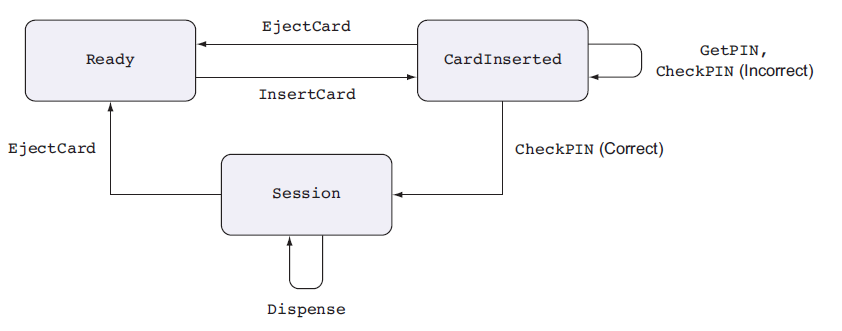
\includegraphics[scale=0.5]{pics/atm-model}
\end{center}
\end{frame}

%%dsl-3
\begin{frame}[fragile]{\dsltitle}
So in our ATM DSL, can be in one of the following states:
\begin{enumerate}
\item[•] \texttt{Ready} — The ATM is ready and waiting for a card to be inserted.
\item[•] \texttt{CardInserted} — There is a card inside the ATM, but the system has not yet checked a PIN entry against the card.
\item[•] \texttt{Session} — There is a card inside the ATM and the user has entered a valid PIN for the card, so a validated session is in progress.
\end{enumerate}
\begin{center}
	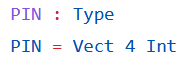
\includegraphics[scale=0.7]{pics/dsl-code-0}
\end{center}
\begin{center}
	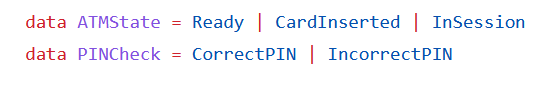
\includegraphics[scale=0.7]{pics/dsl-code-1}
\end{center}
\end{frame}

%%dsl-4
\begin{frame}[fragile]{\dsltitle}
The machine supports the following basic operations:
\begin{enumerate}
\item[•] \texttt{InsertCard} — Waits for a user to insert a card.
\item[•] \texttt{EjectCard} — Ejects a card from the machine, as long as there’s a card in the machine.
\item[•] \texttt{GetPIN} — Reads a user’s PIN, as long as there’s a card in the machine.
\item[•] \texttt{CheckPIN} — Checks whether an entered PIN is valid.
\item[•] \texttt{Dispense} — Dispenses cash as long as there’s a validated card in the machine.
\item[•] \texttt{Message} — Displays a message to the user.
\end{enumerate}
\end{frame}

%%dsl-5
\begin{frame}[fragile]{\dsltitle}
The machine supports the following basic operations:
\begin{center}
	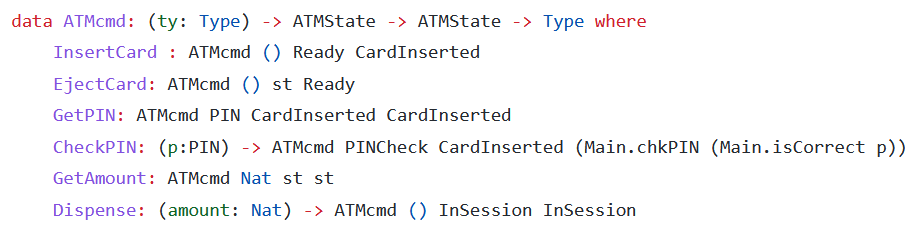
\includegraphics[width=\textwidth]{pics/dsl-code-2}
\end{center}
\end{frame}

%%dsl-6
\begin{frame}[fragile]{\dsltitle}
The machine supports the following basic operations:
\begin{center}
	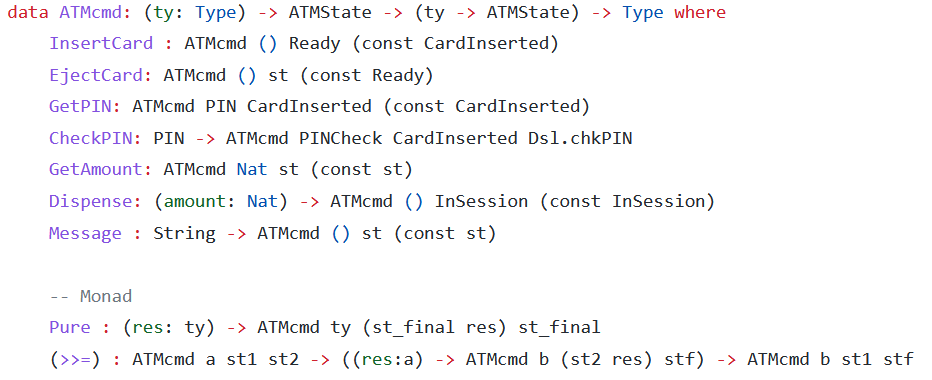
\includegraphics[width=\textwidth]{pics/dsl-code-3}
\end{center}
\end{frame}

%%dsl-7
\begin{frame}[fragile]{\dsltitle}
Its interpreter (part.I)
\begin{center}
	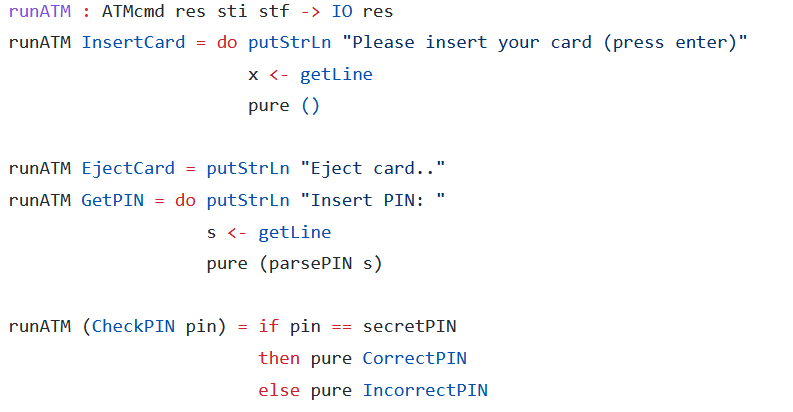
\includegraphics[width=\textwidth]{pics/dsl-code-4_1}
\end{center}
\end{frame}

%%dsl-8
\begin{frame}[fragile]{\dsltitle}
Its interpreter (part.II)
\begin{center}
	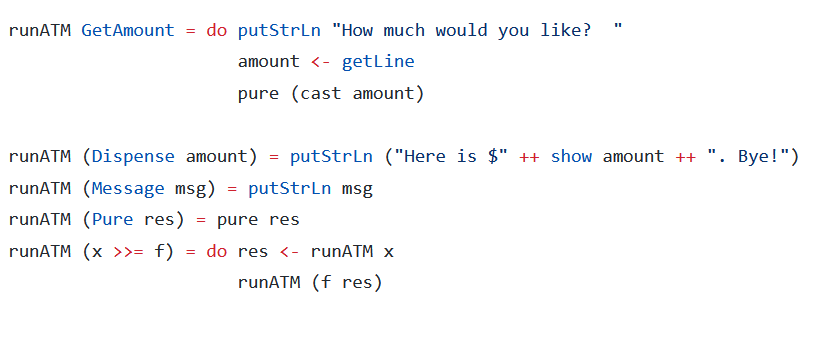
\includegraphics[width=\textwidth]{pics/dsl-code-4_2}
\end{center}
\end{frame}

%%dsl-9
\begin{frame}[fragile]{\dsltitle}
The program. In order to execute it, we have to type in the promt:\\
\texttt{:exec runATM atm}
\begin{figure}
	\raggedright
  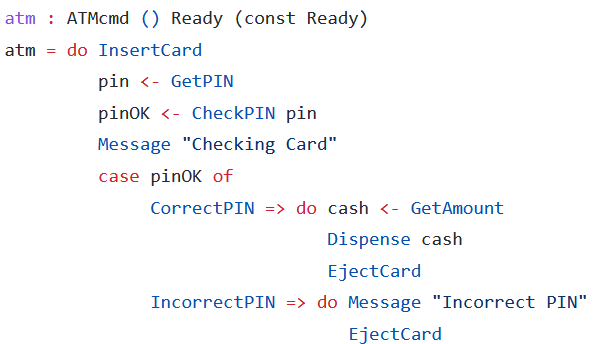
\includegraphics[scale=0.5]{pics/dsl-code-5}
\end{figure}
\end{frame}

%%random-1
\begin{frame}[fragile]{\othertitle}
We can define the following states for our 'mood'
\begin{center}
	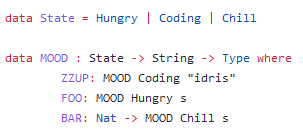
\includegraphics[scale=0.8]{pics/random-code-1}
\end{center}
\end{frame}

%%random-2
\begin{frame}[fragile]{\othertitle}
Let's see what happens..
\begin{figure}
  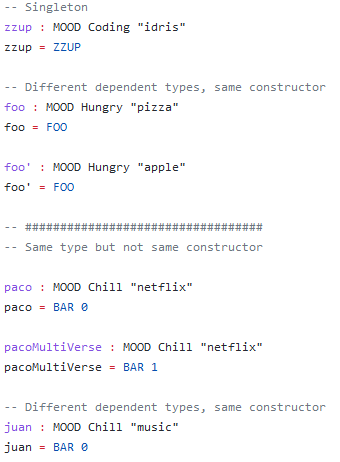
\includegraphics[scale=0.56]{pics/random-code-2}
\end{figure}
\end{frame}


\end{document}

%%% Local Variables:
%%% mode: latex
%%% TeX-master: t
%%% End:
